\documentclass{standalone}
\usepackage{tikz}

\begin{document}
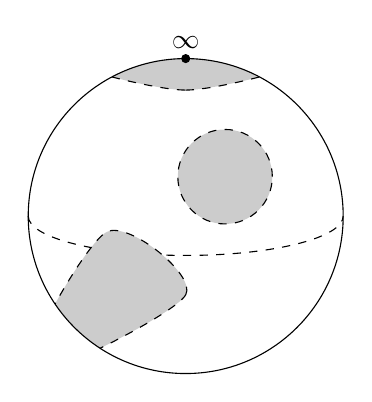
\begin{tikzpicture}
	\draw[dashed] (-2,0) arc[start angle=180, end angle=360, x radius = 2, y
		radius=0.5];
\begin{scope}
\clip (0,0) circle (2);
\filldraw[dashed, fill=gray!40] plot[smooth cycle] coordinates{(-2,-2) (0,-1)
	(-1,-0.2)};
\filldraw[dashed, fill=gray!40] plot[smooth cycle] coordinates{(-1.5,2) (0,1.6)
	(1.5,2)};
\filldraw[dashed, fill=gray!40] (0.5,0.5) circle (0.6);
\end{scope}
\draw (0,0) circle (2);
\filldraw (0,2) circle (0.05) node[above]{$ \infty $};
\end{tikzpicture}
\end{document}

